%- Parkerian Hexag
%- Threats and impacts: un esempio per ogni caso

%Definire un worm
%Diffusione inconsapevole
%Data la facile diffusione si pensava a una propagazione su scala mondiale
%Variante Flame: spio e invio dati a blocchi (per non farmi beccare)
\plain{STUXNET}
\begin{frame}
  \frametitle{Un caso esemplare di attacco: Stuxnet}
  \begin{itemize}[<+- | alert@+>]
  	\item Noto \textbf{\color{blue_slides}worm} di 500 Kbyte scoperto nel 2010 %da VirusBlokAda, una società di sicurezza bielorussa
  	\item Attaccava in 3 fasi:
  	\begin{enumerate}[<+- | alert@+>]
  		\item Attaccava macchine Windows e reti, replicandosi ripetutamente
  		\item Ricercava software Siemens Step7 %Windows-based e utilizzato per programmare sistemi di controllo industriale e infine
  		\item Comprometteva i programmable logic controller
  	\end{enumerate}
  \end{itemize}
  \pause
  \begin{block}{}
  Stuxnet è stato creato e diffuso dal governo USA in collaborazione col governo Israeliano nella centrale iraniana di Natanz
  \end{block}
  \pause
   \begin{block}{Scopo}
   	Sabotare la centrifuga della centrale tramite comandi inviati all’hardware di controllo industriale responsabile della velocità di rotazione delle turbine con l'intento di danneggiarle
   \end{block}
\end{frame}

\begin{frame}{Un caso esemplare di attacco: Stuxnet}
	\begin{figure}[h] 
		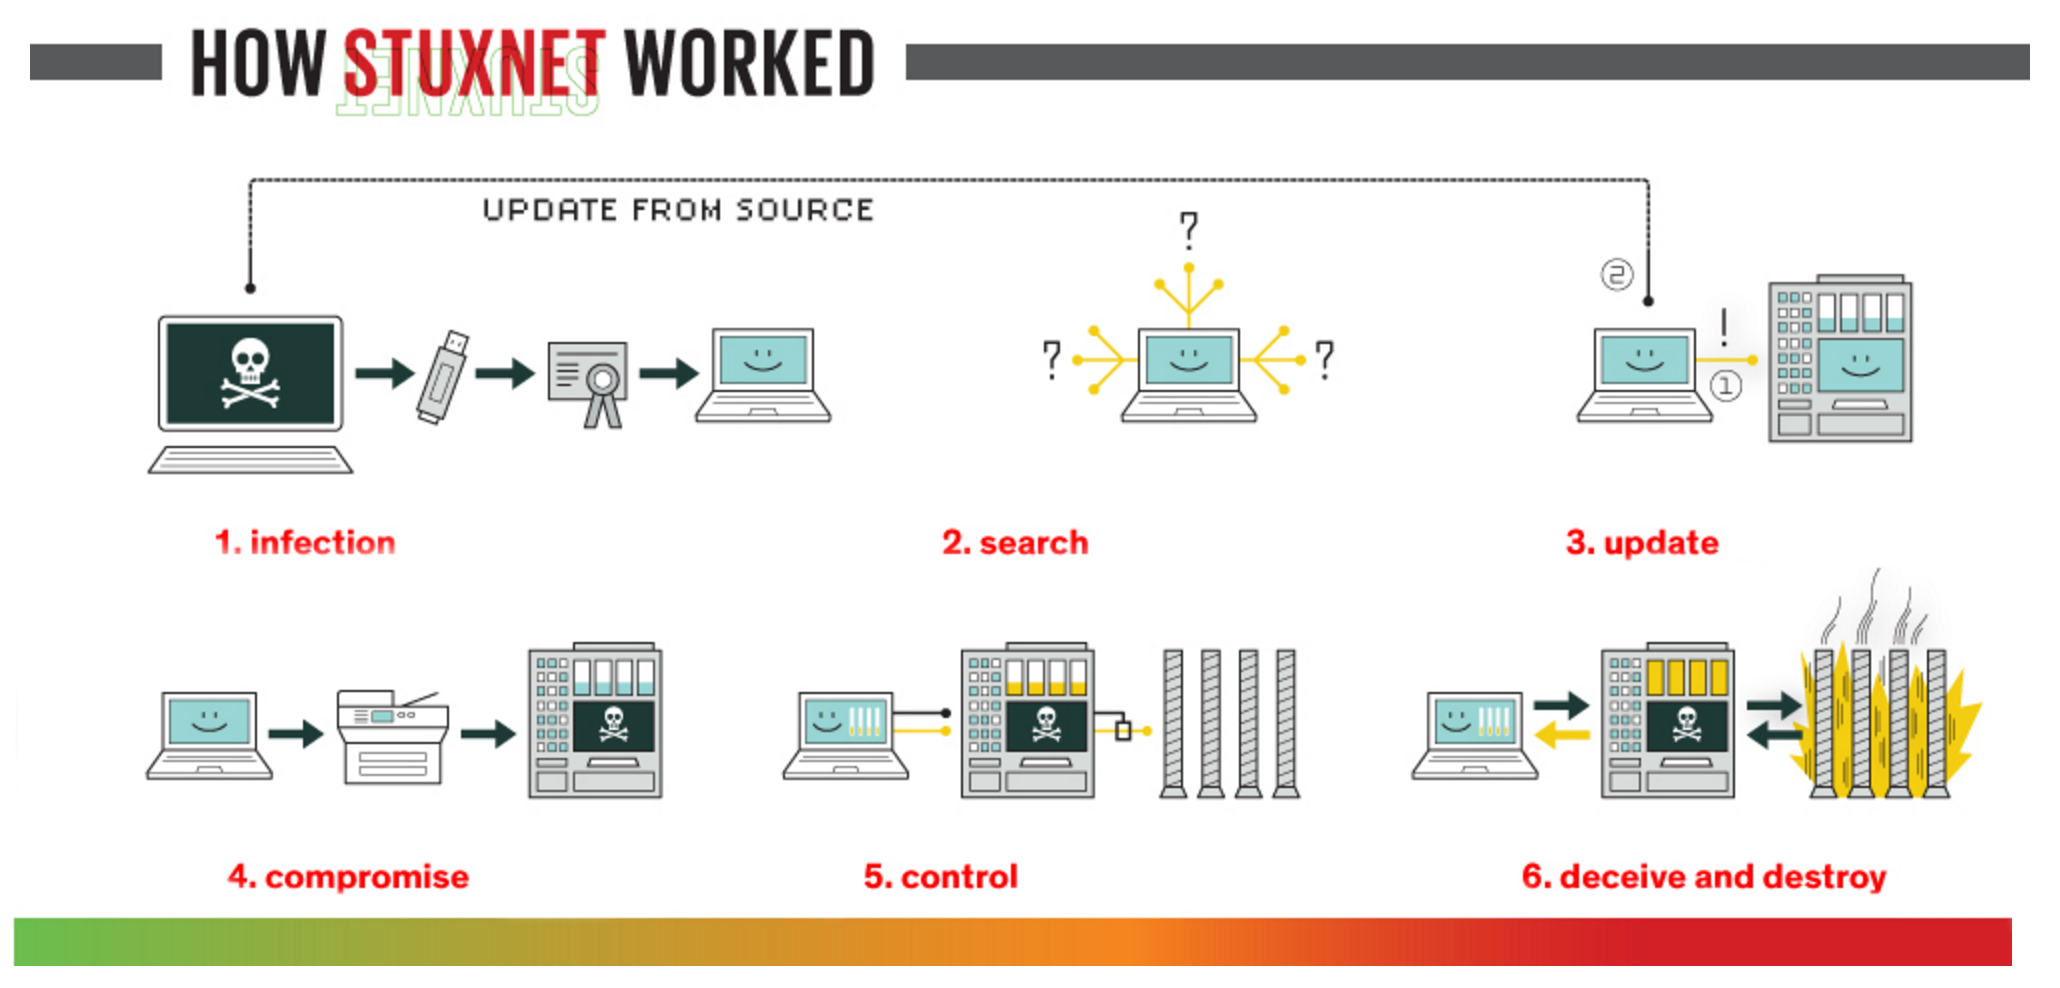
\includegraphics[scale=0.3,cfbox=blue_slides 1pt 0pt]{imgs/stuxnet_hsw.png}
	\end{figure}
\end{frame}
%1. Infection: Entra nel sistema attraverso il collegamento di una penna USB e procede con l’infettare tutte le macchine su cui gira Windows (elude sistemi di automated-detection) (grazie a un certificato digitale che lo fa sembrare affidabile)
%2. Search: Verifica se una macchina è parte del sistema di controllo industriale creato da Siemens
%3. Update: Se il sistema è quello target, il worm accede ad Internet per scaricare una versione più recente di se stesso
%4. Compromise: Compromette i controllori logici del sistema target (sfrutta la vulnerabilità zero-day)
%5. Control: Spia le operazioni del sistema target ed utilizza le informazioni raccolte per prendere il controllo delle centrifughe (portandole al deterioramento)
%6. Deceive & Destroy: Fornisce informazioni fittizie ai controllori assicurandosi che non si accorgeranno del problema

\plain{Definire la sicurezza}

%magari su parkerian hexad parlare delle successive slides senza scriverle
\begin{frame}
  \frametitle{Definire la sicurezza: Parkerian hexad}
  	\begin{figure}[h] 
		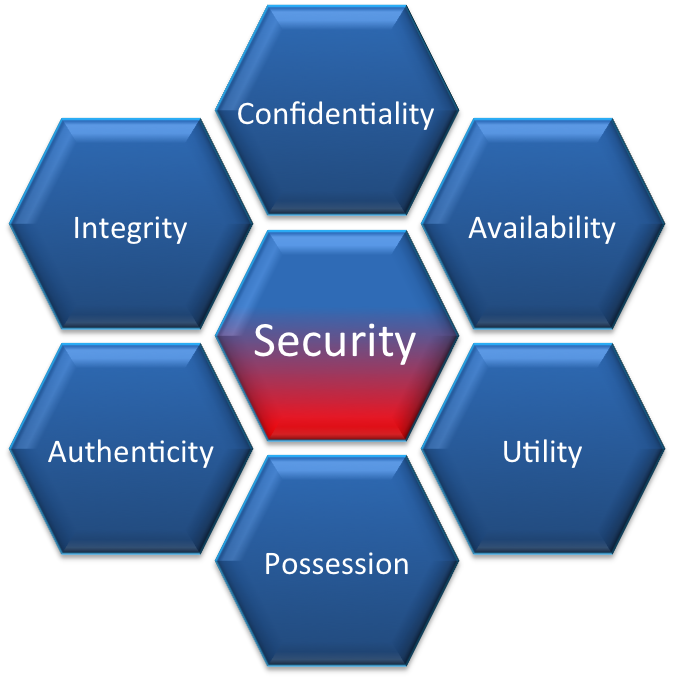
\includegraphics[scale=0.45]{imgs/hexad.png}
		%\caption{Parkerian hexad}
	\end{figure}
\end{frame}

%\begin{frame}
%  \frametitle{Definire la sicurezza}
%  \textbf{Confidentiality}
%  	\begin{itemize}[<+- | alert@+>]
%  		\item Dati confidenziali $\rightarrow$ se noti, potrebbero causare danni alla sicurezza delle operazioni di tutto il sistema
%  		\item Informazioni ricavate dal lavoro delle componenti della Smart Grid
%  		\item Dati personali dei clienti $\rightarrow$ garantire la \textit{privacy}
%  		\item Informazioni aziendali
%  		\item Punti che introducono rischio: locazioni di memoria e meccanismi di trasmissione dati
%  		\item Soluzioni: cifratura dei dati e controllo degli accessi
%  	\end{itemize}
%  %\end{itemize}
%\end{frame}
%
%\begin{frame}
%  \frametitle{Definire la sicurezza}
%   \textbf{Integrity}
%  	\begin{itemize}[<+- | alert@+>]
%  	\item Abilità del sistema di evitare che le informazioni siano modificate da persone o da sistemi non autorizzati
%  	\item Mancanza di integrity $\rightarrow$ il sistema riceve dati non accurati $\rightarrow$ instabilità della Smart Grid
%  	\item Punti che introducono rischio: componenti in cui si consente il passaggio dati da un sistema ad un altro
%  	\item Soluzioni: \textit{auditing}, \textit{authorization}, \textit{nonrepudiation}, \textit{message-signing}
%  	\end{itemize}
%\end{frame}
%
%\begin{frame}
%  \frametitle{Definire la sicurezza}
%   \textbf{Availability}
%  	\begin{itemize}[<+- | alert@+>]
%  	\item Capacità del sistema di compiere il lavoro che gli è stato assegnato, nel momento in cui se ne ha bisogno 
%  	\item Punti che introducono rischio: qualsiasi sistema, rete, dispositivo che gestisce le comunicazioni e che si trova a dover effettuare l'inoltro di un comando da un’estremità del sistema ad un’altra
%  	\item Soluzioni: tecniche di ridondanza
%  	\end{itemize}
%  	\pause
%   \textbf{Control (o Possession)}
%  	\begin{itemize}[<+- | alert@+>]
%  	\item Capacità di controllare le informazioni che necessitano protezione
%  	\item Mancanza di controllo dati $\rightarrow$  compromissione del sistema che li trasmette $\rightarrow$ provenienza delle informazioni non garantita $\rightarrow$ diminuzione dell'affidabilità di quest'ultime
%  	\end{itemize}
%\end{frame}
%
%\begin{frame}
%  \frametitle{Definire la sicurezza}
%   \textbf{Authenticity}
%  	\begin{itemize}[<+- | alert@+>]
%  	\item Processo utilizzato per descrivere la certezza della provenienza
%  	\item Assicurarsi che la fonte dei dati e i dati stessi siano autentici
%  	\end{itemize}
%  	\pause
%  \textbf{Usability (o Utility)}
%  \begin{itemize}[<+- | alert@+>]
%  \item Assicurare che i dati siano utilizzabili
%  \item Flusso di dati cifrato $\rightarrow$ garantisce la sicurezza ma rende difficile far sì che le informazioni siano utili
%  \item Usabilità fornisce valore a livello aziendale $\rightarrow$ trattato come il requisito a più alta priorità
%  \end{itemize}
%\end{frame}

\plain{Building blocks} %una slide con l'elenco e spiegare a voce e magari lasciare quelle sull'integrity

\begin{frame}
  \frametitle{Building blocks}
  \textbf{Layered security model}
  \begin{itemize}
  \item Struttura ad anello 
  \item Comunicazione tra gli strati del sistema sicura
%	  \begin{itemize}
%  	\item Uno strato esterno non può avere libero accesso alle risorse presenti su uno strato più interno
%  	\item Le richieste per le risorse non possono saltare gli anelli
%  	\end{itemize}
  \item Assicurare che un fallimento in uno strato non abbia impatto nè in uno strato più basso nè in qualsiasi sistema dello stesso strato
  \end{itemize}
    	\begin{figure}[h] 
		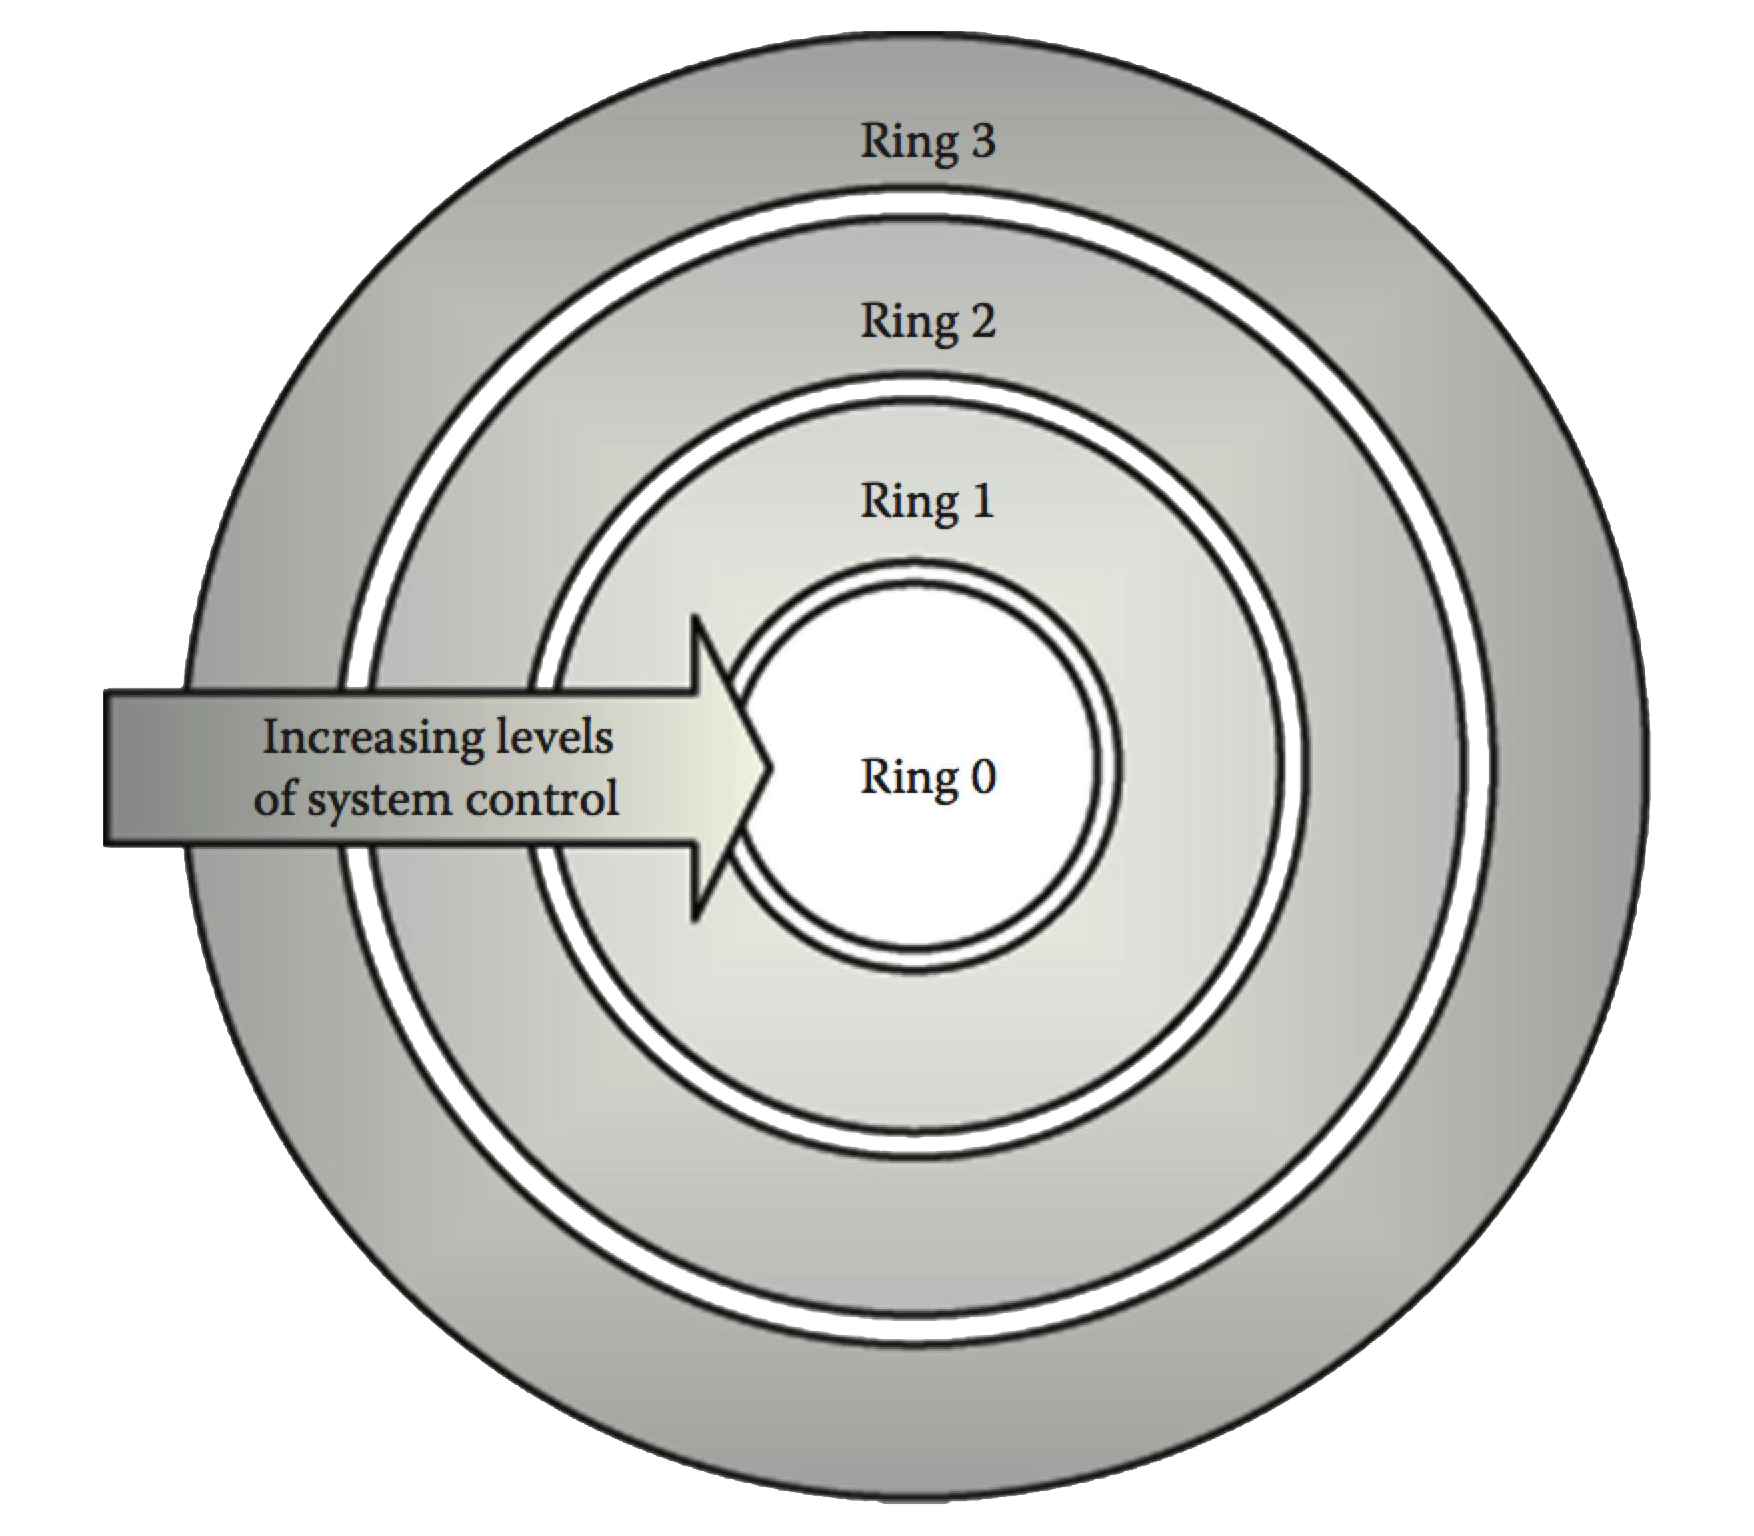
\includegraphics[scale=0.1]{imgs/ring.png}
	\end{figure}
\end{frame}


%magari togliere per tutti il puntino più esterno
\begin{frame}
  \frametitle{Building blocks}
  \begin{itemize}[<+- | alert@+>]
  \item Authentication
%  \begin{itemize}[<+- | alert@+>]
%  \item Processo di verifica dell'identità di una persona o di un servizio che richiede l'accesso ad una risorsa
%  \item Autenticazione non solo per l'utente ma anche tra sistemi, processi o componenti hardware
%  \end{itemize}
 \item Authorization
% 	\begin{itemize}
% 		\item Verifica di ciò che la persona o il servizio autenticato può fare all'interno del contesto del sistema
% 	\end{itemize}
	\item Auditing
	\item Key management
  \end{itemize}
\end{frame}

%\begin{frame}
%  \frametitle{Building blocks}
%  \begin{itemize}[<+- | alert@+>]
%  \item \textit{Auditing}
%  \begin{itemize}
%  \item Revisione periodica dell'efficacia dei meccanismi di sicurezza della Smart Grid
%  \item Testing delle componenti essenziali per mettere in sicurezza le operazioni
%  \end{itemize}
% \item \textit{Key management}
% 	\begin{itemize}
% 		\item Processo di gestione dell'emissione delle chiavi per utenti, applicazioni e dispositivi
% 		\item Utilizzate per stabilire l'identità dell'utente e garantire l'integrità dei messaggi
% 		\item Impiego di Public Key Infrastructure
% 	\end{itemize}
%  \end{itemize}
%\end{frame}

\begin{frame}
  \frametitle{Building blocks}
  \begin{itemize}[<+- | alert@+>]
  \item Message integrity
  \begin{itemize}
  \item Signing
  	\begin{itemize}
  	\item Messaggio inviato da un sistema ad un altro $\rightarrow$ autenticazione $\rightarrow$ autorizzazione $\rightarrow$ scambio di messaggi
  	\end{itemize}
  \item Nonrepudiation
    \begin{itemize}
  	\item Mittente riconosciuto tramite una prova inconfutabile della sua identità
  	\end{itemize}
  \item Encryption
    \begin{itemize}
  	\item Messaggio non può essere letto da una persona/sistema non diretto destinatario
  	\end{itemize}
 	\end{itemize}
  \end{itemize}
\end{frame}

\begin{frame}
  \frametitle{Building blocks}
  \begin{itemize}[<+- | alert@+>]
  \item Network integrity
  \begin{itemize}
  \item Firewall
  \item Rilevamento e prevenzione delle intrusioni
 	\end{itemize}
   \item System integrity
     \begin{itemize}
  \item Protezione da malware
  \item Gestione della configurazione del sistema
  \item Validazione e testing
 	\end{itemize}
  \end{itemize}
\end{frame}

\plain{Threats and Impacts}%minacce una slide

\begin{frame}
  \frametitle{Threats and Impacts: Consumer threats}
  \begin{itemize}[<+- | alert@+>]
  \item Minacce naturali
	\begin{itemize}
	\item Venti, tempeste, tornadi e terremoti
%	\item Eliminare totalmente i danni causati da tali calamità non è possibile
%	\item Di critica importanza la definizione di programmi di aiuto in caso di incidenti
	\end{itemize}
	 \item Minacce da singoli o da organizzazioni
	\begin{itemize}
	\item Ladri e stalker
	\item Hacker
	\item Terrorismo
	\item Governo
	\item Società di servizi, in particolare i lavoratori
	\end{itemize}
  \end{itemize}
\end{frame}

%\begin{frame}
%  \frametitle{Threats and Impacts: Consumer threats}
%  \begin{itemize}[<+- | alert@+>]
%  \item \textit{Minacce da singoli o da organizzazioni}
%	\begin{itemize}
%	\item Ladri e stalker
%	\item Hacker
%	\item Terrorismo
%	\item Governo
%	\item Società di servizi, in particolare i lavoratori
%	\end{itemize}
%  \end{itemize}
%\end{frame}

%%%%meno testo, più parole chiave da qui in giù. Parole tolte usate a voce

\begin{frame}
  \frametitle{Threats and Impacts: Consumer threats - Impatti}
	\textbf{Privacy del consumatore}
		\begin{itemize} [<+- | alert@+>]
		\item Raccolta di informazioni personali
		\item Attaccante può utilizzarli per scopi malevoli
		\end{itemize}
	\textbf{Impatto sull'availability}
			\begin{itemize} [<+- | alert@+>]
		\item Obiettivo Smart Grid: disponibilità perenne di corrente
		\item Attacchi possono causare: alterazione di termostati, limitazione di servizi d'emergenza
		\end{itemize}
	\textbf{Impatto finanziario}
				\begin{itemize} [<+- | alert@+>]
		\item Corruzione di dati $\rightarrow$ emissione di bollette inaccurate
		\end{itemize}
\end{frame}

\begin{frame}
  \frametitle{Threats and Impacts: Utility companies threats}
  \textit{Confidentiality}
  \begin{itemize}[<+- | alert@+>]
	  \item Privacy del consumatore
	  \begin{itemize}
	  \item Attacco alla Web application della società 
	  \item Analisi dello storico dei consumi $\rightarrow$ identificare comportamenti utente
	  \end{itemize}
	\item Informazioni proprietarie
		\begin{itemize}
		\item Segreto aziendale $\rightarrow$ target appetibile per hacker
		\end{itemize}
 	\end{itemize}
\end{frame}

\begin{frame}
  \frametitle{Threats and Impacts: Utility companies threats}
  \textit{Integrity}
  \begin{itemize}[<+- | alert@+>]
	  \item Frode
	  \begin{itemize}
	  \item Manomissione dello smart meter per sottostimare i consumi $\rightarrow$ bollette meno costose 
	  \item Modifica dati relativi alla produzione di energia $\rightarrow$ compensi maggiori
	  \end{itemize}
	\item Manipolazione dei dati dei sensori
		\begin{itemize}
		\item Simulare un guasto $\rightarrow$ la società spende tempo e denaro per le riparazioni
		\end{itemize}
 	\end{itemize}
\end{frame}

\begin{frame}
  \frametitle{Threats and Impacts: Utility companies threats}
  \textit{Availability}
  \begin{itemize}[<+- | alert@+>]
	\item Clienti
	  	\begin{itemize}
	  	\item Connessione allo smart meter di un utente $\rightarrow$ cambio password + spegnimento corrente
	  	\end{itemize}
	\item Organizzazioni
			\begin{itemize}
			\item Hacker che vuole danneggiare la società $\rightarrow$ \textit{Denial of Service attack}
			\item Ex dipendente di un'azienda
			\end{itemize}
	\item Manipolazione del mercato
		\begin{itemize}
		\item Team di hacker + esperti di mercati finanziari $\rightarrow$ Ottenere significative quantità di denaro in poco tempo
		\end{itemize}
 	\end{itemize}
\end{frame}
